Thinking...
The user asks: "以下のの日本語文を英訳してください。ただしTeXのコードが挿入されているのでその部分はそのまま出力してください：" Then they give a LaTeX figure environment. So we need to translate the Japanese text while preserving the LaTeX code unchanged. The Japanese text appears to be only the caption: "5年ごとの収録論文数". Also maybe the surrounding text? The whole snippet includes figure environment with caption. So we need to output the same LaTeX code but with caption translated into English. Should we translate "5年ごとの収録論文数" to "Number of papers collected every 5 years" or "Number of papers recorded every five years". Probably "Number of papers collected per 5-year interval". We'll choose "Number of papers collected every 5 years". Also maybe translate "figure" environment? No, keep code unchanged except caption text.

Thus output:

\begin{figure}[h]
\begin{center}
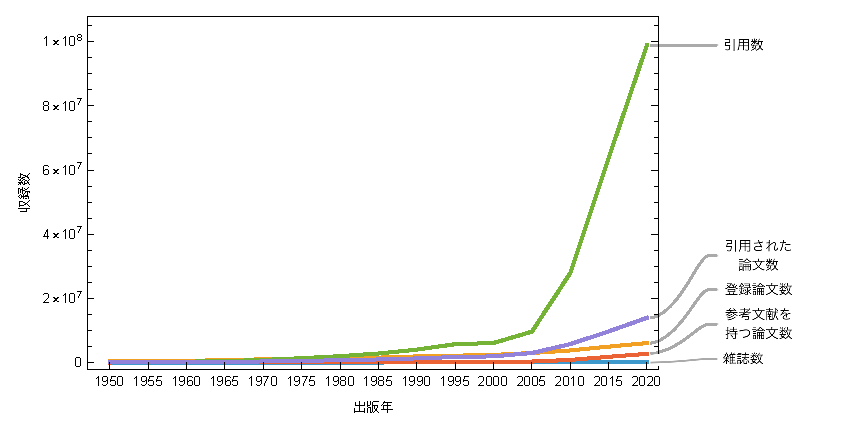
\includegraphics[width=76mm]{gr2.eps}
\caption{Number of papers collected every 5 years}
\label{fig:gr2}
\end{center}
\end{figure}

Provide as answer.
...done thinking.

\begin{figure}[h]
\begin{center}
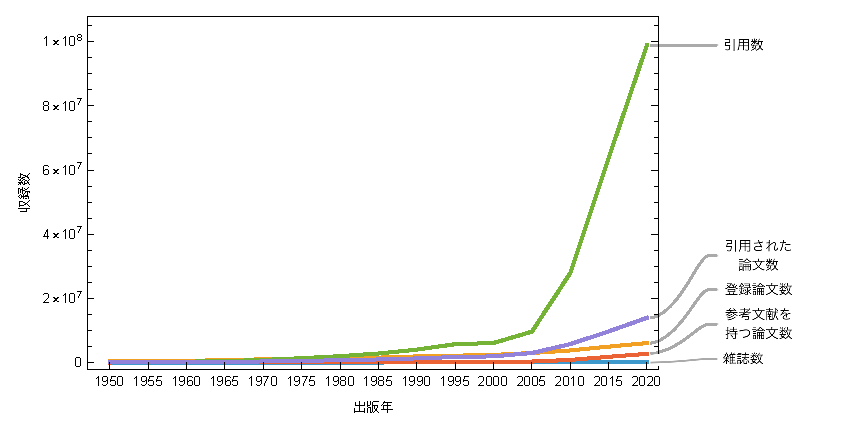
\includegraphics[width=76mm]{gr2.eps}
\caption{Number of papers collected every 5 years}
\label{fig:gr2}
\end{center}
\end{figure}

